\documentclass{beamer}
\usepackage{ctex, hyperref}
\usepackage[T1]{fontenc}

% other packages
\usepackage{latexsym,amsmath,xcolor,multicol,booktabs,calligra}
\usepackage{graphicx,pstricks,listings,stackengine}

\author{Balint Armand Alexandru,\\
Barna Tudor Cristian,\\
Screciu Alin Constantin}
\title{Tutorial on Java Modelling Language}
\subtitle{An introductive tutorial}
\institute{West University of Timisoara}
\date{06.02.2022}
\usepackage{Style}

% defs
\def\cmd#1{\texttt{\color{red}\footnotesize $\backslash$#1}}
\def\env#1{\texttt{\color{blue}\footnotesize #1}}
\definecolor{deepblue}{rgb}{0,0,0.5}
\definecolor{deepred}{rgb}{0.6,0,0}
\definecolor{deepgreen}{rgb}{0,0.5,0}
\definecolor{halfgray}{gray}{0.55}

\lstset{
    basicstyle=\ttfamily\small,
    keywordstyle=\bfseries\color{deepblue},
    emphstyle=\ttfamily\color{deepred},    % Custom highlighting style
    stringstyle=\color{deepgreen},
    numbers=left,
    numberstyle=\small\color{halfgray},
    rulesepcolor=\color{red!20!green!20!blue!20},
    frame=shadowbox,
}


\begin{document}

\kaishu
\begin{frame}
    \titlepage
    \begin{figure}[htpb]
        \vspace*{-0.5cm}
        \begin{center}
            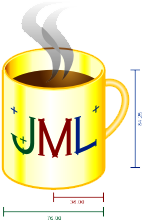
\includegraphics[width=1.5cm,height=2.3cm]{pic/jml-logo-med.png}
        \end{center}
    \end{figure}
\end{frame}

\begin{frame}
    \tableofcontents[sectionstyle=show,subsectionstyle=show/shaded/hide,subsubsectionstyle=show/shaded/hide]
\end{frame}


\section{What is JML?}

\begin{frame}{What is JML?}
    \begin{itemize}[<+-| alert@+>]
        \item JML, short for "Java Modelling Language", is a behavioral interface specification language designed to specify Java classes and methods.
        \item It is heavily based on syntactic sugar to make various notations
        \item It uses mathematical concepts in order to describe the behavior of a module without providing the concrete implementation details
        \item It can be written either inside the code or in the documentation.
    \end{itemize}
\end{frame}


\section{Why use JML?}

\begin{frame}{Why should you use JML?}
    \begin{itemize}[<+-| alert@+>]
        \item It is easy to read and deduce its meaning!
        \item Provides runtime assertion checking, which also helps in automating parts of testing
        \item Helps in verifying if the described specifications are fulfilled.
        \item Even its lightweight specifications can help bug-seeking tools
    \end{itemize}
\end{frame}


\section{JML vs Other specification languages}

\subsection{Comparison between JML and other SLs}

\begin{frame}{Advantages of JML}
    \begin{itemize}
        \item Besides the ease of read, JML is made exclusively for Java
        \item JML gives the important benefit of being able to specify exceptions; a vital feature for Java code
        \item Methods can be called from assertions ( e.g. $//@ \textbackslash ensures (members < getMaxMembers()$ ) 
        \item It can be written directly into the source code
        
    \end{itemize}
\end{frame}

\subsection{Code Snippets}

\begin{frame}{VDM-SL vs JML}

Below will be 2 different code snippets, namely VDM-SL and JML
\bigskip

    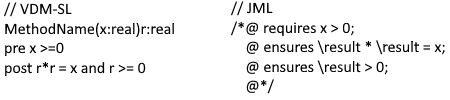
\includegraphics[height=60pt,width=300pt]{pic/code1.png}

As we can see, both code snippets refer to the same squaring method for real numbers and JML is much tidier than VDM-SL

\end{frame}

\subsection{Tools for JML}

\begin{frame}{What are JML tools good for?}
    Pertaining to JML tools, there is a plethora of options, yet all of them share some of the features, those being:
    \begin{itemize}
        \item typo-checker
        \item a type-checker to find any assertions which refer to fields which no longer exist together
        \item annotation parsing
    \end{itemize}
\end{frame}

\begin{frame}{What are JML tools good for?}
    And for some more specific tools:
    \begin{itemize}
        \item \textbf{jmlc} - runtime assertion checking \& assertion violation guard%which handles the runtime assertion checking and is on the lookout for JML assertion violations
        \item \textbf{jmlunit} - similar but combined with unit testing%accomplishes mainly the same thing but also combined with unit testing
        \item \textbf{jmlspec} - helps the user generate JML specifications%which helps the user generate JML specifications
        \item \textbf{Daikon} - detects possible invariants%that detects possible invariants by observing the runtime behaviour of the program
        \item \textbf{Houdini} - uses Java to deduce annotations for code
    \end{itemize}
\end{frame}

\section{Basics of JML}

\subsection{Bare-bones structure}



\begin{frame}{Bare-bones structure}
        JML specifications imply that all the methods of a particular data type ensure an outcome as long as the conditions are satisfied\\ \medskip% work by the "design by contract" philosophy which means that all the methods of a particular data type ensure an expected outcome if the conditions are satisfied\\ \medskip
        Preconditions are specified using the "\textit{requires}" clause and postconditions via the "\textit{ensures}" clause.\\ \medskip
        Throughout the code if we need to use an invariant, we can do so by using the "\textit{invariant}" keyword.\\ \medskip
        
\end{frame}

\begin{frame}{Bare-bones structure example}
The JML annotations which are contained inside the Java source code, are put inside comments that start with the symbol "@" \\ \bigskip
        \centering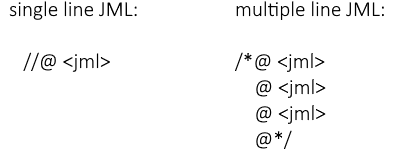
\includegraphics[width=8.5cm,height=3cm]{pic/jmlstruc.png}
\end{frame}

\subsection{JML Annotations}
\begin{frame}{JML Annotations}
    Just like Java, JML also have multiple types of annotations, some examples being:
    \begin{itemize}
        \item Modifiers - "\textbf{pure}" , "\textbf{spec\_public}" , "\textbf{helper}" and so on.%. Modifiers are single words such as \textbf{pure}, \textbf{spec\_public} and \textbf{helper}. They are syntactically similar to Java modifiers like "\textit{public}" and "\textit{static}"
        
        \item Clauses%. A JML clause begins with a keyword, such as ensures, followed by an expression or other information and ending with a semicolon.
        \item Types - "\textbf{\textbackslash real}", "\textbf{\textbackslash bigint}", etc.%. JML defines a number of new specification-only types, such as \textbf{\textbackslash real} and "\textbf{\textbackslash bigint}"
        \item Expression tokens - can be either single words like \textbf{\textbackslash result} or function-like, such as \textbf{\textbackslash old(x)}%. These occur within JML expressions. They begin with a backslash and they can be either single words like \textbf{\textbackslash result} or function-like, such as \textbf{\textbackslash old(x)}
    \end{itemize}
\end{frame}

\subsection{Annotation placement}

\begin{frame}{Annotation placement}
    These annotations are generally located above the method they specify, similar to invariants, which are also usually placed before the fields it mentions. Example below\\
    \bigskip
    \centering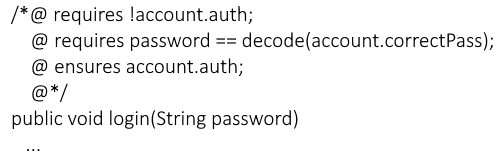
\includegraphics[width=8.5cm,height=3cm]{pic/jmllogin.png}
\end{frame}

\subsection{Heavyweight vs Lightweight}
\begin{frame}{Lightweight vs Heavyweight}
    In JML, specifications can be either \textbf{lightweight} or \textbf{heavyweight}. Lightweight specifications are where the user specifies only what they deem as important. For the unspecified attributes, both specifications give default values however the heavyweight expects the user to know the default values as they are not as forgiving.
\end{frame}

\begin{frame}[fragile]{Lightweight vs Heavyweight}
     In order to go from a lightweight specification to a heavyweight one, the user must include this at the beginning of the annotation:
    \begin{lstlisting}
[optional privacy modifier] behavior-keyword
    \end{lstlisting}
    Where "\textit{behavior-keyword}" should be replaced by behavior, normal\_behavior or exceptional\_behavior
\end{frame}

\subsubsection{Lightweight example}
\begin{frame}[fragile]{Lightweight example}
    \begin{lstlisting}
public abstract class Light {
protected boolean init_state, end_goal;
protected int helper;
/*@
  @ requires init_state;
  @ assignable helper;
  @ ensures end_goal;
  @*/
protected abstract int some_method();
}        
    \end{lstlisting}
   
\end{frame}

\subsubsection{Heavyweight example}
\begin{frame}[fragile]{Heavyweight example}
    \begin{lstlisting}
public abstract class LightAsHeavy {
protected boolean init_state, end_goal;
protected int helper;
/*@ protected behavior
  @ requires init_state;
  @ diverges false;
  @ assignable helper;
  @ working_space \not_specified;
  @ ensures end_goal;
  @ signals_only \nothing;
  @ signals \not_specified;
  @*/
protected abstract int someMethod();
}       
    \end{lstlisting}
   
\end{frame}

\subsection{Default return values of unspecified clauses}
\begin{frame}{Default return values of unspecified clauses}

A fairly important detail is how there are different default values for unspecified clauses. These are determined by the type of specification they are a part of. The listing will specify first the lightweight first and heavyweight second.

\end{frame}

\begin{frame}{Default return values of unspecified clauses}
\begin{itemize}
    \item \textbf{requires} \& \textbf{ensures}. "\textbackslash \textit{not\_specified}" - "\textit{true}"
    \item \textbf{diverges}. "\textit{false}" for both.
    \item \textbf{assignable}. "\textbackslash \textit{not\_specified}" - "\textbackslash \textit{everything}" 
    \item \textbf{accessible}. "\textbackslash \textit{everything}" for both.
    \item \textbf{callable}. "\textbackslash \textit{everything}" for both.
    \item \textbf{working\_space}. "\textbackslash \textit{not\_specified}" for both.
    \item \textbf{signals\_only}. "\textbackslash \textit{nothing}" for both.
    \item \textbf{signals}. "\textbackslash \textit{not\_specified}" - "\textit{true}"
    \item \textbf{when}. "\textbackslash \textit{not\_specified}" - "\textit{true}"


\end{itemize}
\end{frame}





\section{Implementing JML}
\subsection{Bare-bones structure}
\begin{frame}{How to start implementing JML into your programs}
To write JML specifications we need to place them into specially formatted Java comments. This means that a Java compiler will ignore the JML text. JML specifications have to be written in comments that either
\begin{enumerate}
    \item begin with "\textit{//@ }"
    \item begin with "\textit{/*@ }" and end with "\textit{@*/}"
    
\end{enumerate}
\end{frame}

\begin{frame}[fragile]{How to start implementing JML into your programs}
It is common practice for lines within such a block comment to have the first non-whitespace characters be a series of @ symbols followed by a space. 
\begin{lstlisting}
public class ClassName {
    /*@ requires requirement1;
      @ ensures assurance;
      @*/
    void method() { ... }
}
\end{lstlisting}
\end{frame}

\subsection{Implementing JML for BubbleSort}
\begin{frame}{Implementing JML for BubbleSort}
Let us take Bubble Sort as an example method. This method takes one argument, namely an array, which must not be NULL. Therefore, below the declaration of the method and above the first line of code, we have to specify a precondition using the requires keyword.    
\end{frame}

\begin{frame}[fragile]{}
\begin{lstlisting}
public class BubbleSort {    
 //@ requires arr != null;
 public static void sort(int [] arr) {        
   for (int i = 0; i < arr.length; i++) {
     for (int j = arr.length-1; j > i; j--) {
       if (arr[j-1] < arr[j]) {
         int tmp = arr[j];
         arr[j] = arr[j-1];
         arr[j-1] = tmp;
         }
       }
     }
   }
 }
\end{lstlisting}
\end{frame}

\begin{frame}{}
However, we will not stop here. This method should sort the given array, which means that we will also have to add a postcondition using the ensures keyword and due to that, we must also change the comment from a single line to a multiple line one.
\end{frame}

\begin{frame}[fragile]{}
\begin{lstlisting}[basicstyle=\footnotesize]
public class BubbleSort {    
/*@
  @ requires arr != null; 
  @ ensures \forall int k; 0 <= k && k < arr.length -1;
  @           arr[k] > arr[k+1];
  @*/
 public static void sort(int [] arr) {        
   for (int i = 0; i < arr.length; i++) {
     for (int j = arr.length-1; j > i; j--) {
       if (arr[j-1] < arr[j]) {
          int tmp = arr[j];
          arr[j] = arr[j-1];
          arr[j-1] = tmp;
         }
       }
     }
   }
 }
\end{lstlisting}
\end{frame}

\begin{frame}{}
With the method definition done, we shall now move into the insides of the method. However, worth noting is that we use the \textbackslash forall expression which in the given example will increment k by one, as long as it satisfies the given bounds.
\end{frame}

\begin{frame}[fragile]{}
\begin{lstlisting}[]
public static void sort(int [] arr) {        
  /*@ final ghost int n = arr.length;   
    @ loop_invariant 0 <= i <= n;
    // elements up-to i are sorted
    @ loop_invariant \forall int k; 0<= k < i; 
    @               \forall int l; k < l < n; 
    @                arr[k] >= arr[l];
    @ decreasing n-i;
    @*/
  for (int i = 0; i < arr.length; i++) {
     for (int j = arr.length-1; j > i; j--) {
       if (arr[j-1] < arr[j]) {
         int tmp = arr[j];
         arr[j] = arr[j-1];
         arr[j-1] = tmp;
       }
    }
  }
}
\end{lstlisting}
\end{frame}

\begin{frame}{}
We now have arranged the first loop too, therefore we can move onto the second. But, before that, we can see that in the scope above, a ghost variable has been used. A ghost variable is one that can only be accessed inside of the particular specification and it does not necessarily mirror a value of the class, nor of the method. The decreasing keyword signifies that the "$n-i$" calculation will decrease after every iteration and will be different from zero.
\end{frame}

\begin{frame}[fragile]{}
\begin{lstlisting}[]
for (int i = 0; i < arr.length; i++) {
  /*@ loop_invariant i <= j <= n-1; 
    // j-th element is always the largest
    @ loop_invariant \forall int k; j <= k < n;
    @               arr[j] >= arr[k]; 
    // elements up-to i remain sorted
    @ loop_invariant \forall int k; 0 <= k < i;
    @                \forall int l; k < l < n; 
    @                arr[k] >= arr[l]; 
    @ decreasing j;
    @*/
     for (int j = arr.length-1; j > i; j--) {
       if (arr[j-1] < arr[j]) {
         int tmp = arr[j];
         arr[j] = arr[j-1];
         arr[j-1] = tmp;
        }
      }
}
\end{lstlisting}
\end{frame}

\begin{frame}{}
And with that, our implementation of JML in the BubbleSort algorithm is now complete and ready to be ran.
\end{frame}

\section{Conclusion}

\begin{frame}{Miscellaneous}
    The presentation you have been given comes alongside a paper on JML which goes over the same aspects but in more detail. In addition, the full BubbleSort JML code and another example with a more in-depth insight will be found in there together with a well-explained step-by-step tutorial on how to set up JML.
\end{frame}

\begin{frame}[<+->]{Conclusion}
    To conclude, we will be answering a very common question:\\
    \medskip
    \begin{itemize}
        \item "\textit{Should I use JML?}"
    \end{itemize}
    \smallskip
    And the answer to that is \textbf{Yes!}\\
    \medskip
    Unlike a decade ago, needs for tools to fix mismanagement of and wrongly implemented code have arisen and in furtherance of future large scale projects, of which code has to be proven correct before execution or launch, it is recommended to consider specification languages such as JML.
\end{frame}

\begin{frame}{}
    \begin{center}
        {\Huge Thank you for your attention.}
    \end{center}
\end{frame}

\end{document}